In this section we study the performance of various jet algorithms in
combination with jet substructure variables/taggers in terms of the
identification of a boosted hadronically decaying $W$ signal. For each
jet algorithm we produce Receiver Operating Characteristic (ROC)
curves that elucidate the performance of various variables that are
capable of providing discrimination between a hadronic $W$ signal and
a QCD jet. These variables are then combined in a Boosted Decision Tree (BDT) and the performance of the resulting BDT discriminant
explored through ROC curves to understand the degree to which
variables are correlated and exploiting the same information. These
studies are repeated in different kinematic regimes, to explore both
the performance and correlations as a function of the jet boost, and
where substructure approaches may break down.

\subsection{Methodology}

These studies use the $X \rightarrow WW$ samples as signal and the XXX
samples to model the QCD background. 

Jets are reconstructed using the XXX jet algorithms described in the
previous section. The following event selection is then applied to these
samples....(presumably this will vary depending on which kinematic bin
is used, as will the actual samples used - maybe summarize in a table).

Show some basic distributions of the background versus signal -
groomed jet pT, groomed jet mass for the different
algorithms. Figure~\ref{fig:pt500_basics_AKt_R08} shows these basic
distributions. {\it Do we want to reweight signal kinematics to
background or vice versa? Do we want to study quarks/gluons separately?}

Go on to explain how we produce the ROC curves.

\begin{figure*}
\begin{center}
\subfigure[Leading jet
\pT]{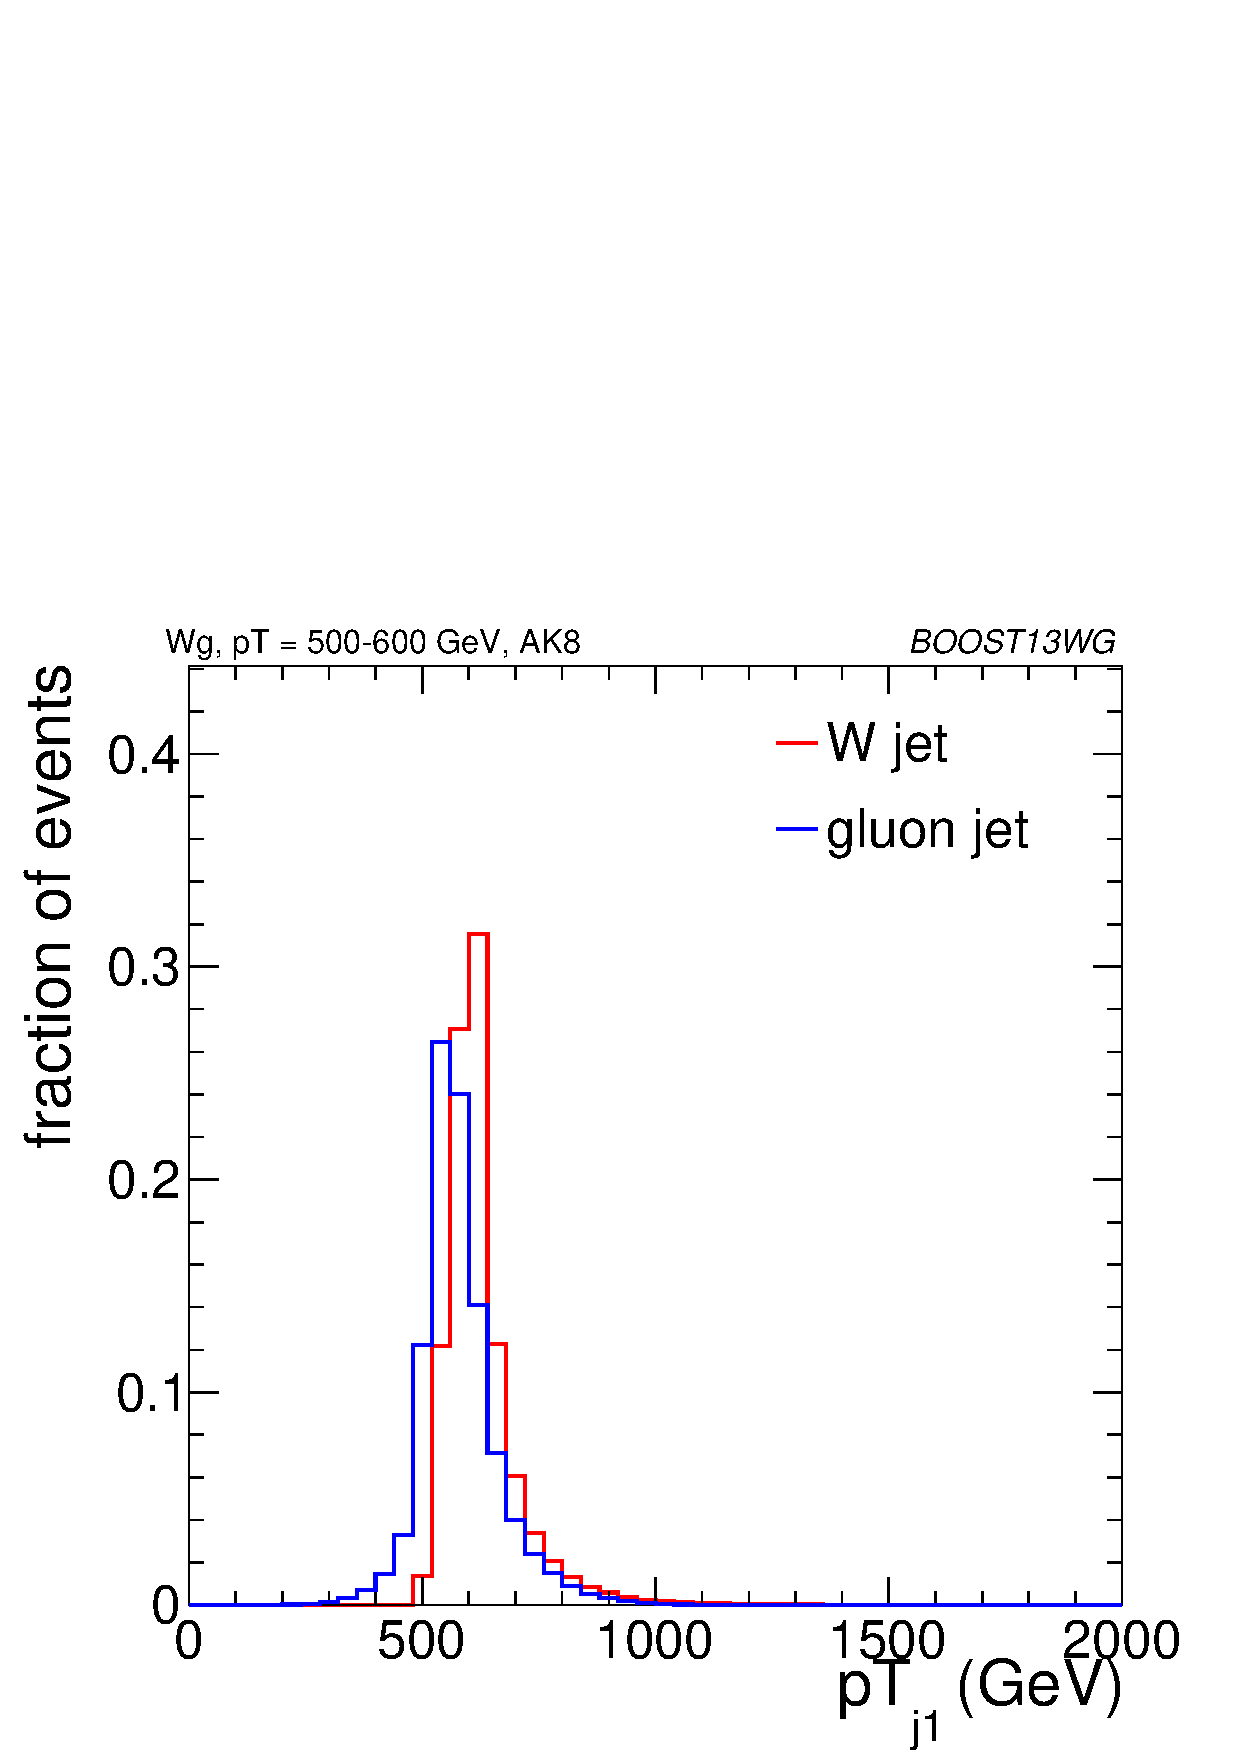
\includegraphics[width=0.48\textwidth]{./Figures/WTagging/pT500/AKtR08/jpt1.png}}
\subfigure[Sub-leading jet
\pT]{\includegraphics[width=0.48\textwidth]{./Figures/WTagging/pT500/AKtR08/jpt2.png}}
\subfigure[Leading jet
$\eta$]{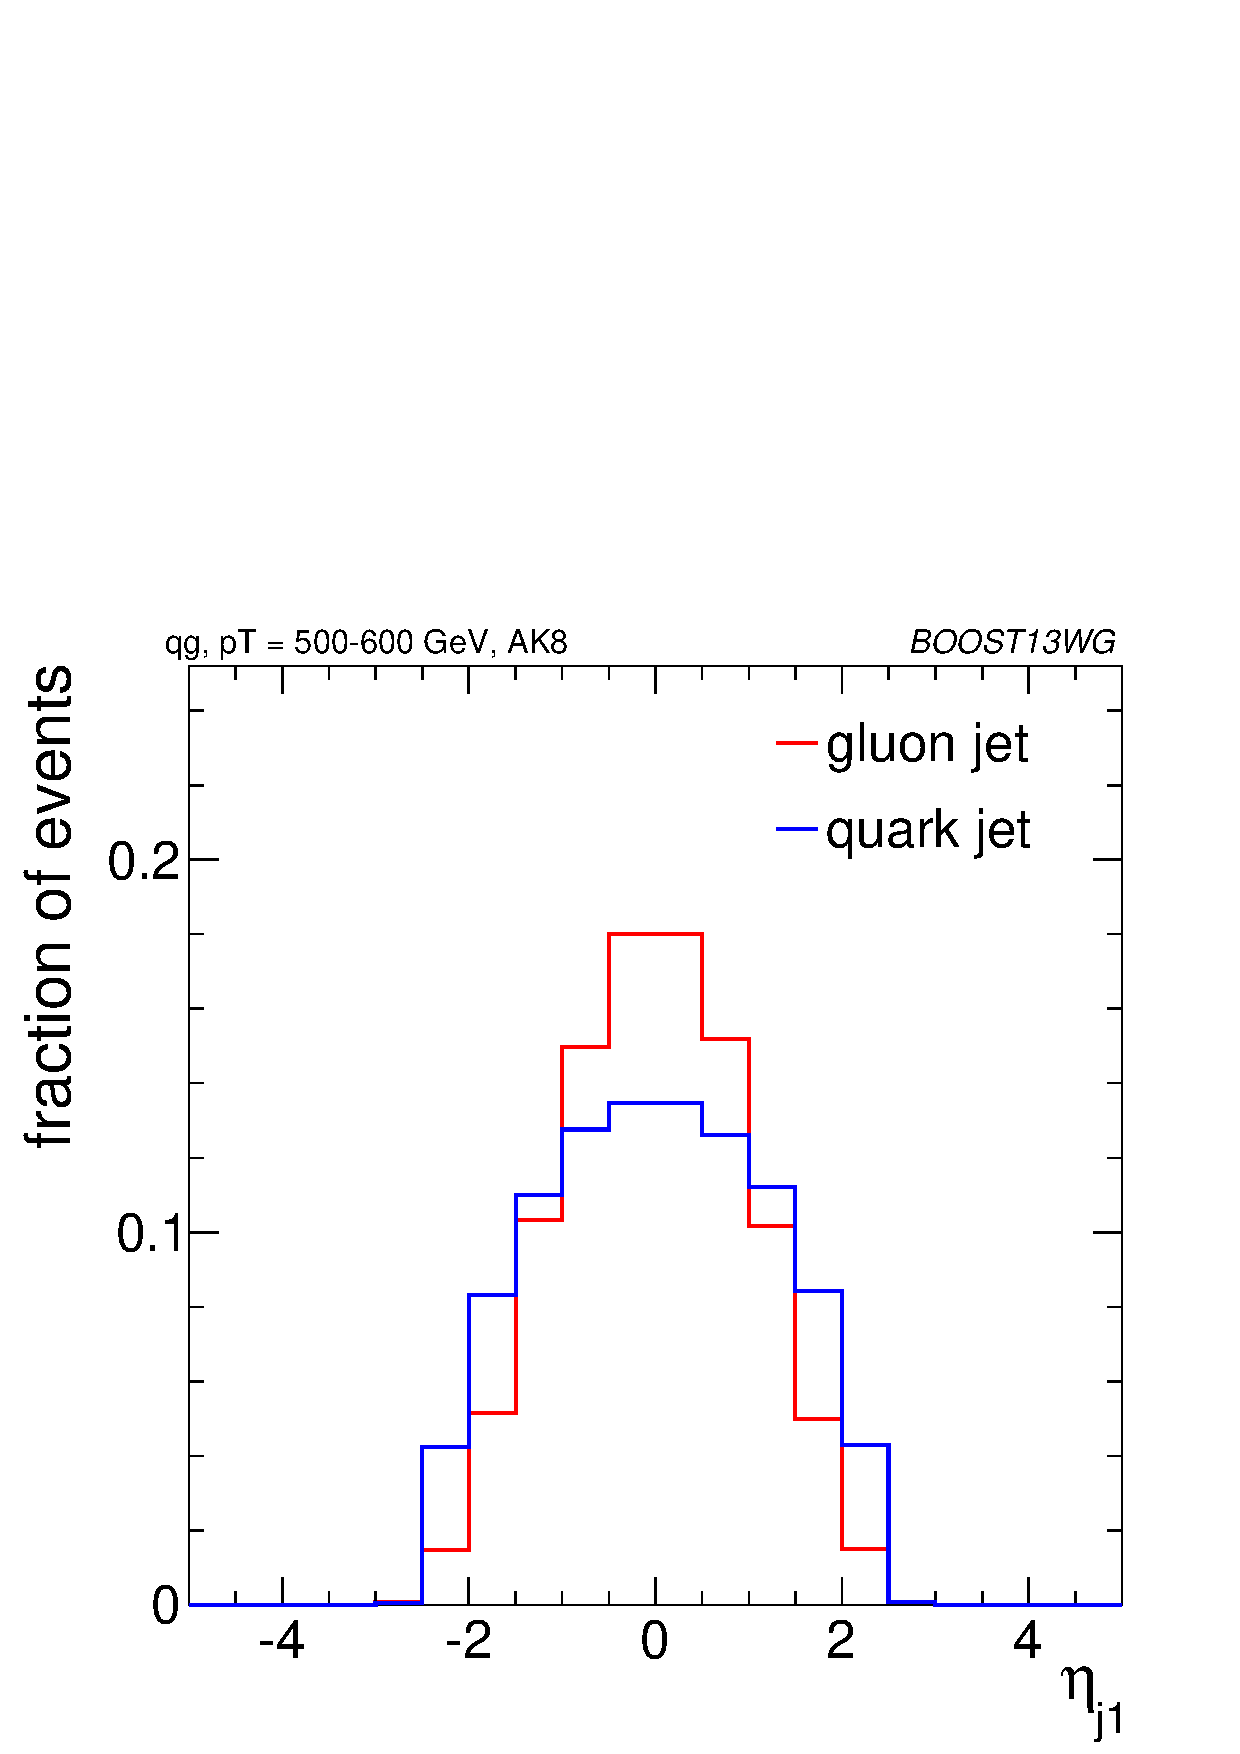
\includegraphics[width=0.48\textwidth]{./Figures/WTagging/pT500/AKtR08/jeta1.png}}
\subfigure[Sub-leading jet
$\eta$]{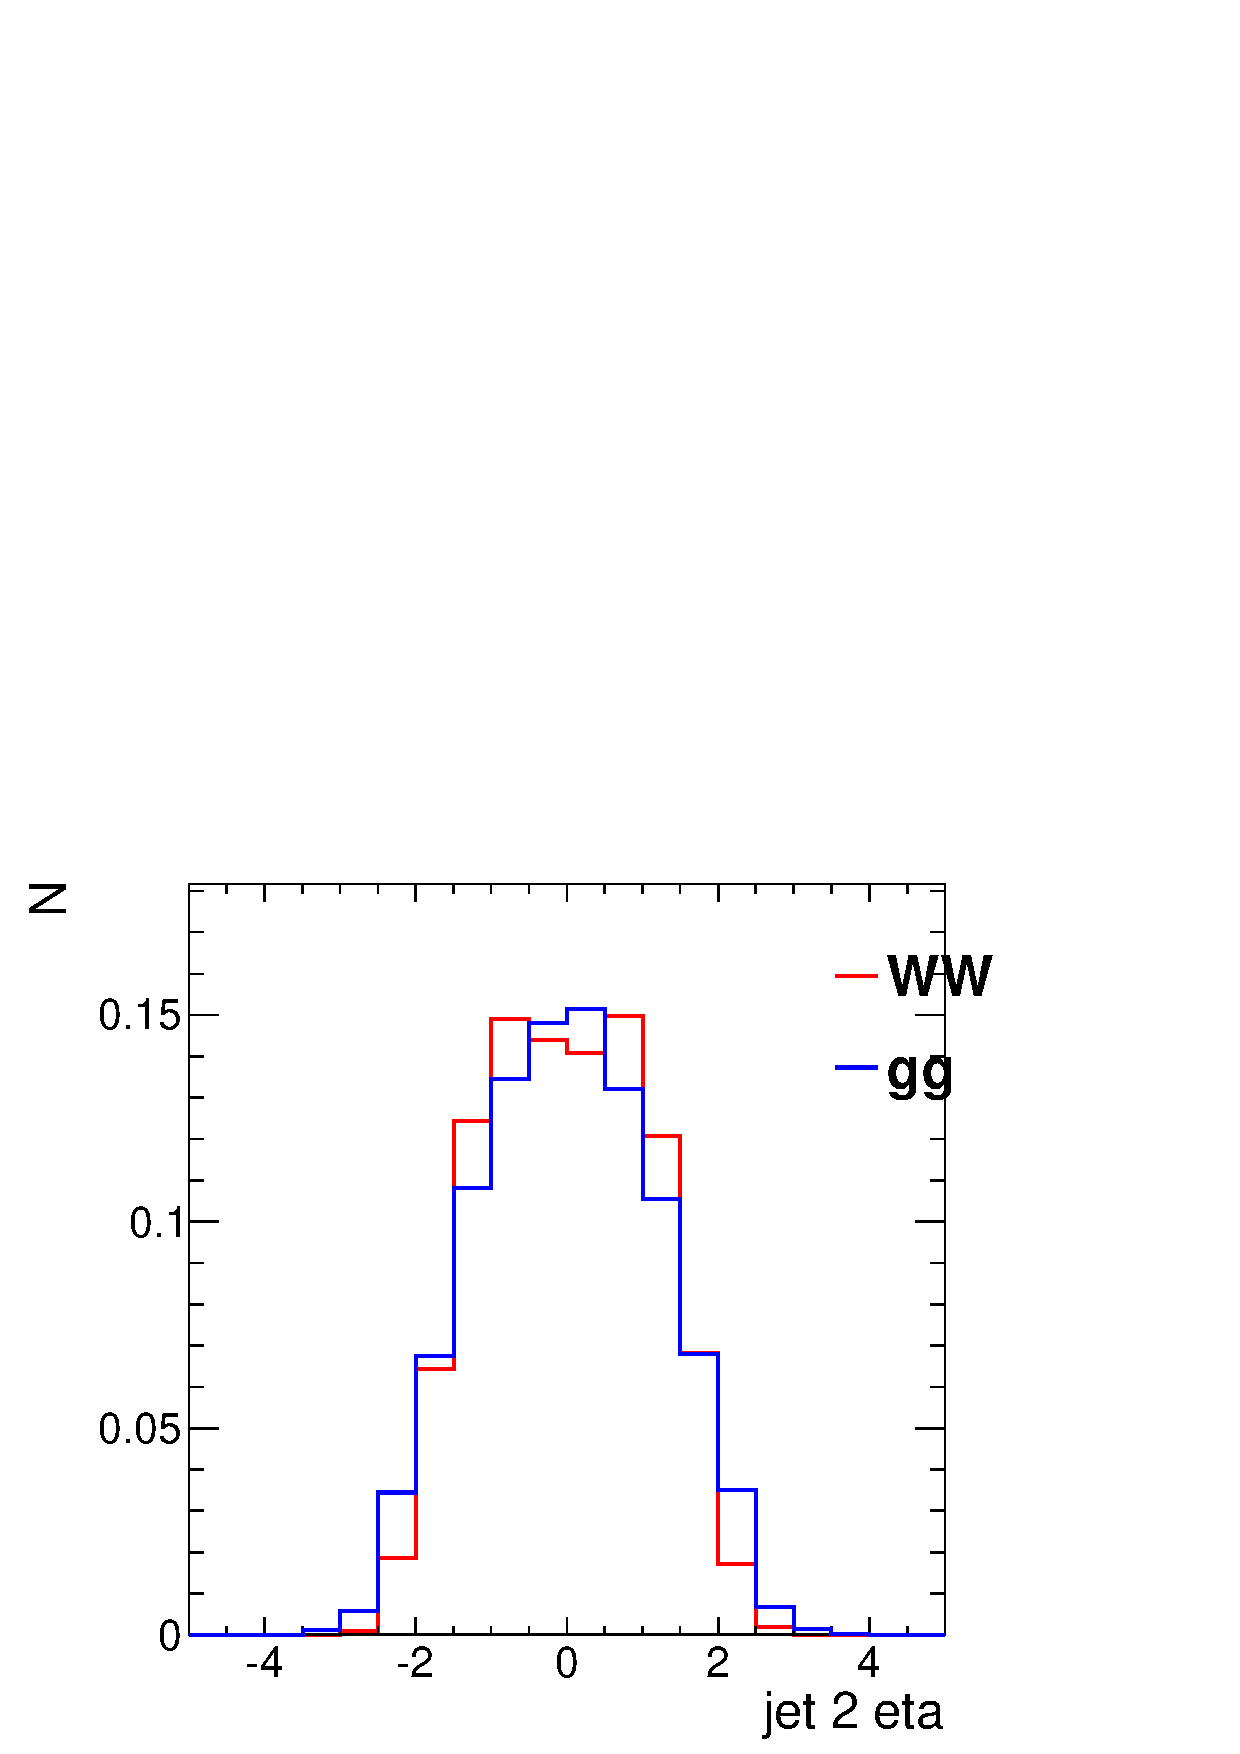
\includegraphics[width=0.48\textwidth]{./Figures/WTagging/pT500/AKtR08/jeta2.png}}

\caption{The BDT combinations of each mass variable with every other
variable considered in the \pt 500 GeV bin using the anti-\kT R=0.8 algorithm.}
\label{fig:pt500_basics_AKt_R08}
\end{center}
\end{figure*}

\subsection{Performance at Moderate Boosts}

(this section is to cover the $W$-tagging performance for jet \pT 200-300 GeV and
500-600 GeV using $\sqrt{s} = 8$ TeV samples)

\subsubsection{Single Variable Performance}

{\it Show plots of signal versus background for all single variables investigated}.

Figure~\ref{fig:pt500_single_AKt_R08} shows the single variable ROC curves in
the \pT 500 GeV bin for the anti-\kT R=0.8 algorithm, compared to the
ROC curve for a BDT combination of all the variables. One can see that
the best performant single variables for a reasonable signal
efficiency are the groomed/filtered masses, which all have a similar
level of performance with the exception of the soft drop mass with $\beta=-1$. {\it Would be good to split this into two plots, one
using the masses and one for other variables, or somehow make the mass
and other variable curves more distinct from one another by using same
colour for all the mass curves}.

{\it We want to look also at:
\begin{itemize}
\item Dependence on R. So have the same single variable ROC for
e.g. R=1.2, R=0.4. Then possibly have another plot which compares the
best single variable (e.g. groomed mass) for
different R.
\item Dependence on pT. Again want to repeat the plot for different
kinematic bins, and then have a plot which compares the best
performance in each kinematic bin to see the dependence of performance
on kinematics.
\end{itemize}
}

\begin{figure*}
\begin{center}
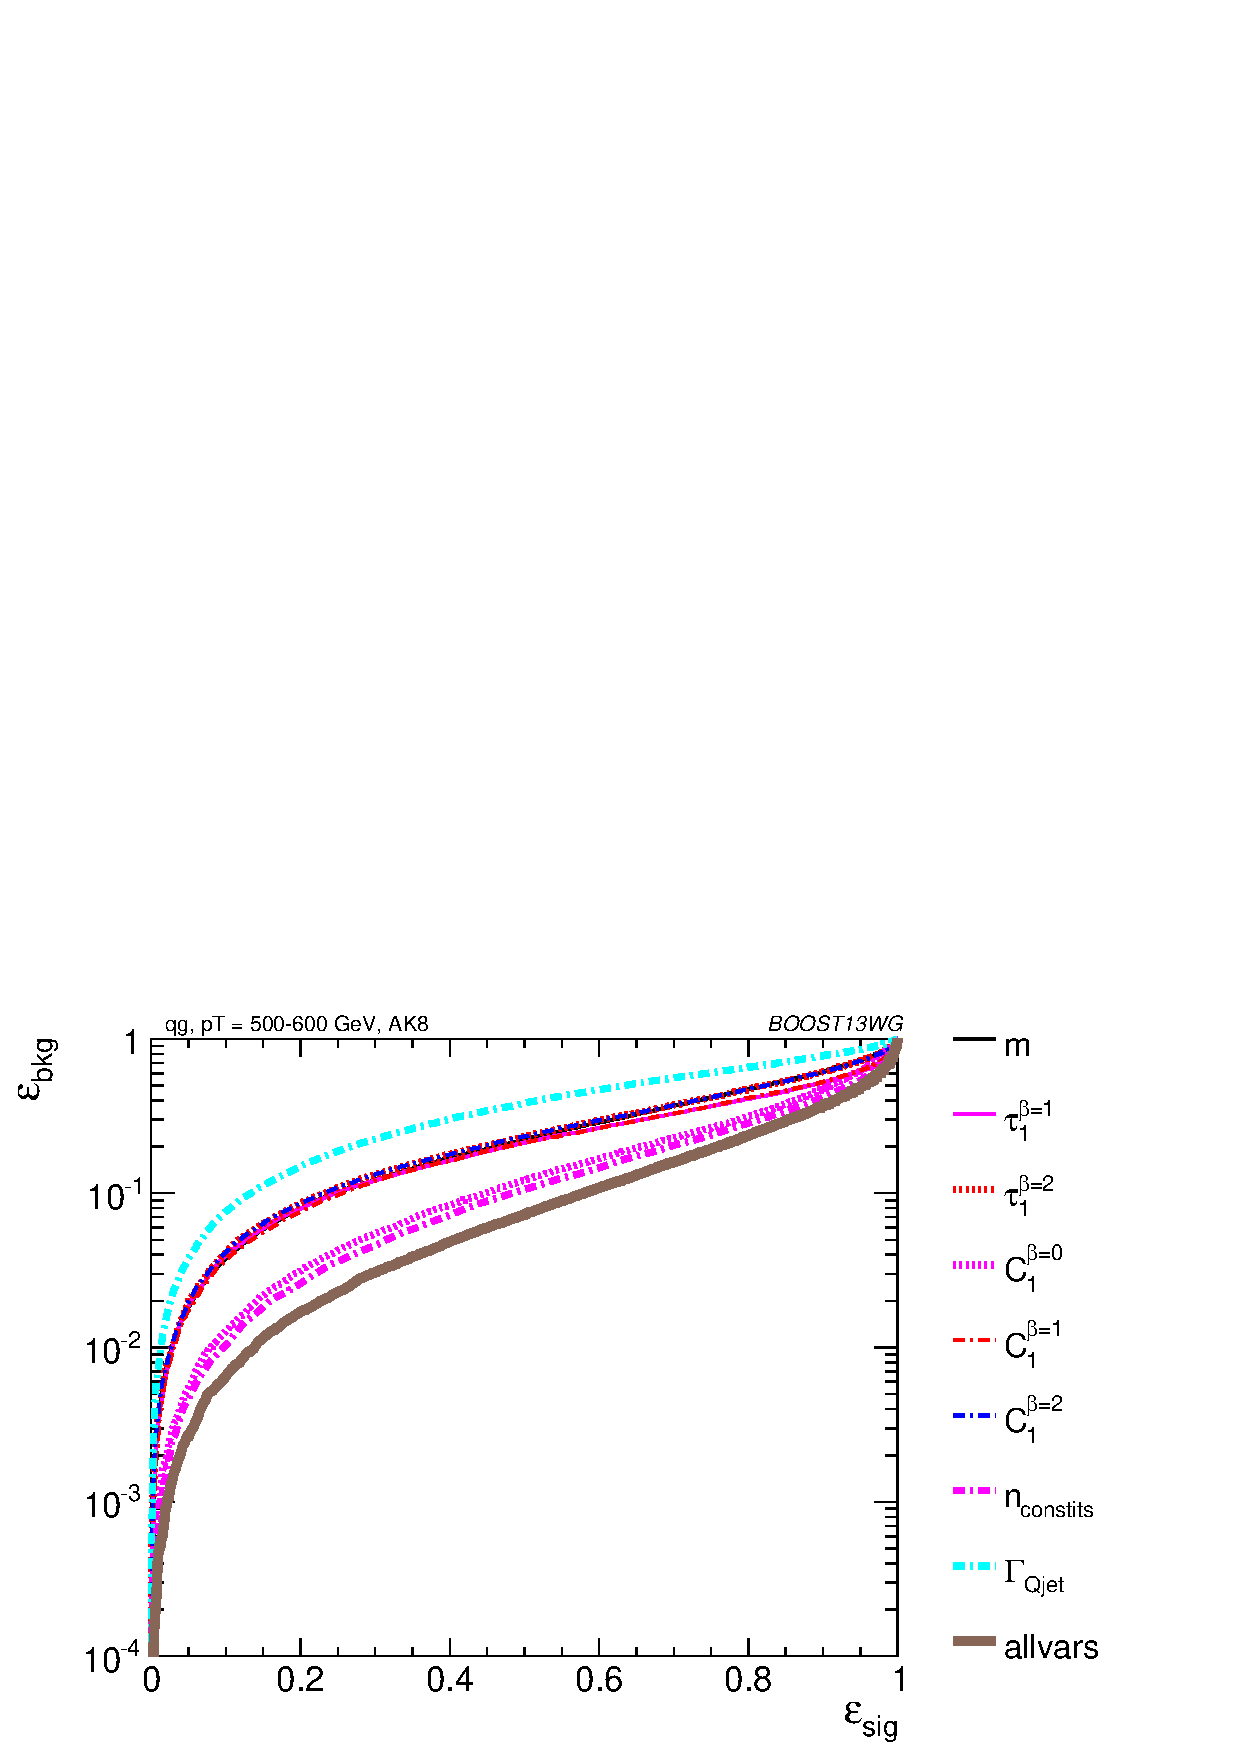
\includegraphics[width=0.8\textwidth]{./Figures/WTagging/pT500/AKtR08/Rocs_1D_single.png}
\caption{The ROC curve for all single variables considered for $W$
tagging in the \pt 500 GeV bin using the anti-\kT R=0.8 algorithm.}
\label{fig:pt500_single_AKt_R08}
\end{center}
\end{figure*}

\subsubsection{Combined Performance}

Figure~\ref{fig:pt500_masscomb_AKt_R08} shows the BDT combinations of each mass variable with every other
variable considered in the \pt 500 GeV bin using the anti-\kT R=0.8
algorithm. {\it Can we drop the combinations of mass + mass
from these plots to make them clearer? Also would be good to put the
single variable mass curve on these plots, so you can see how much
improvement the combination gives, and the ``all variables'' curve.}

No combination with other variables can recover the poor performance
of the ungroomed mass and the soft drop mass with $\beta=-1$. The
other groomed/filtered masses are all most improved by combination
with the $C_{2}^{\beta=1}$ energy correlation function. {\it Show 2-D
correlation plot of $C_{2}^{\beta=1}$ vs groomed mass - show that it
is largely uncorrelated.}
{\it Now show a plot which compares on one plot the best combined performance for
each mass + X. e.g. mass + $C_{2}^{\beta=1}$, and compared also to the
all variables curve. This plot is just for
one R and one kinematic bin.}

{\it Repeat these studies for different R and different kinematic
bins. Finally make plots which compare best combined performance for
different R and kinematics.}

{\it Do we want to look at other combinations of variables which don't
involve mass? Practically I think we will always be making mass + X though.}

\begin{figure*}
\begin{center}
\subfigure[Ungroomed mass + X]{\includegraphics[width=0.48\textwidth]{./Figures/WTagging/pT500/AKtR08/Rocs_1D_jmass.png}}
\subfigure[Trimmed mass + X]{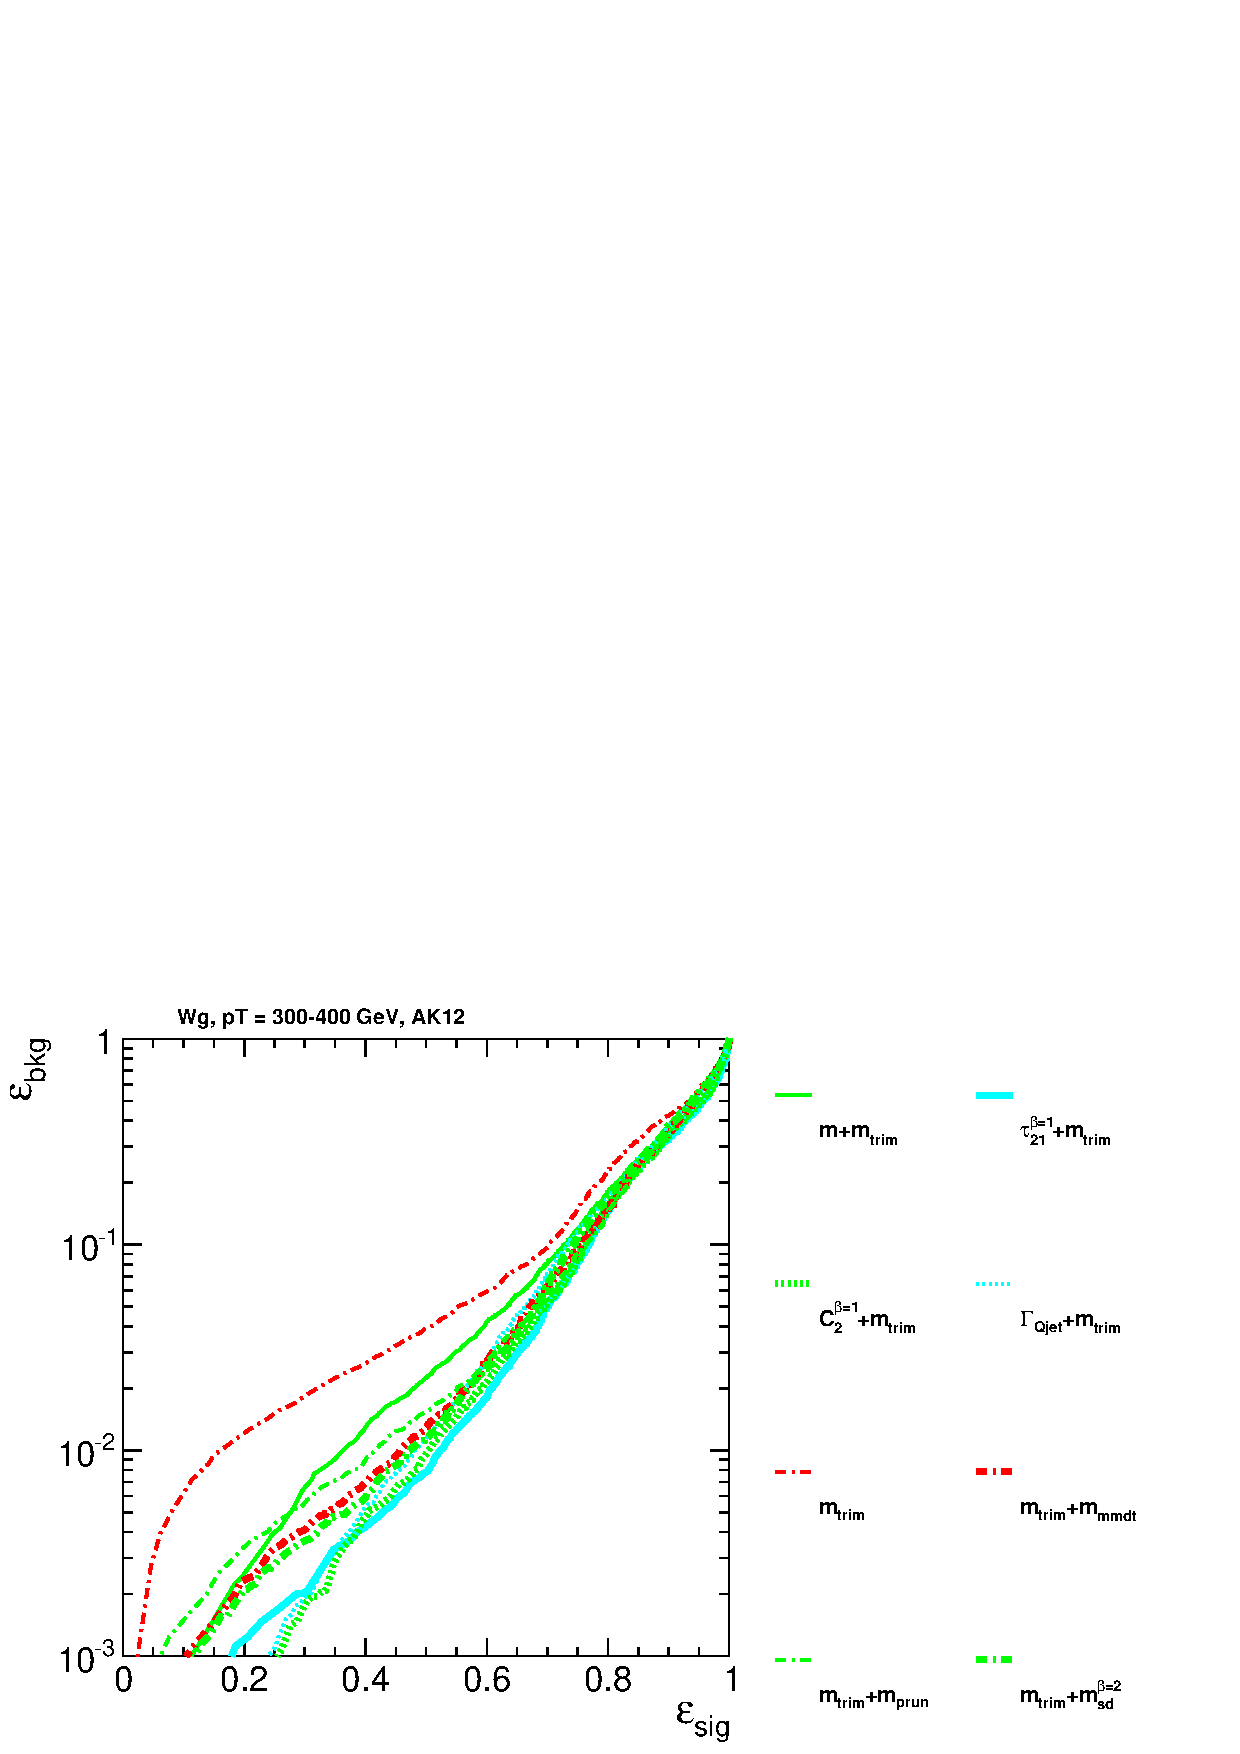
\includegraphics[width=0.48\textwidth]{./Figures/WTagging/pT500/AKtR08/Rocs_1D_j_mass_trim.png}}
\subfigure[Pruned mass + X]{\includegraphics[width=0.48\textwidth]{./Figures/WTagging/pT500/AKtR08/Rocs_1D_j_mass_prun.png}}
\subfigure[Soft drop mass ($\beta=-1$) +X]{\includegraphics[width=0.48\textwidth]{./Figures/WTagging/pT500/AKtR08/Rocs_1D_j_mass_sdm1.png}}
\subfigure[Soft drop mass ($\beta=2$) + X]{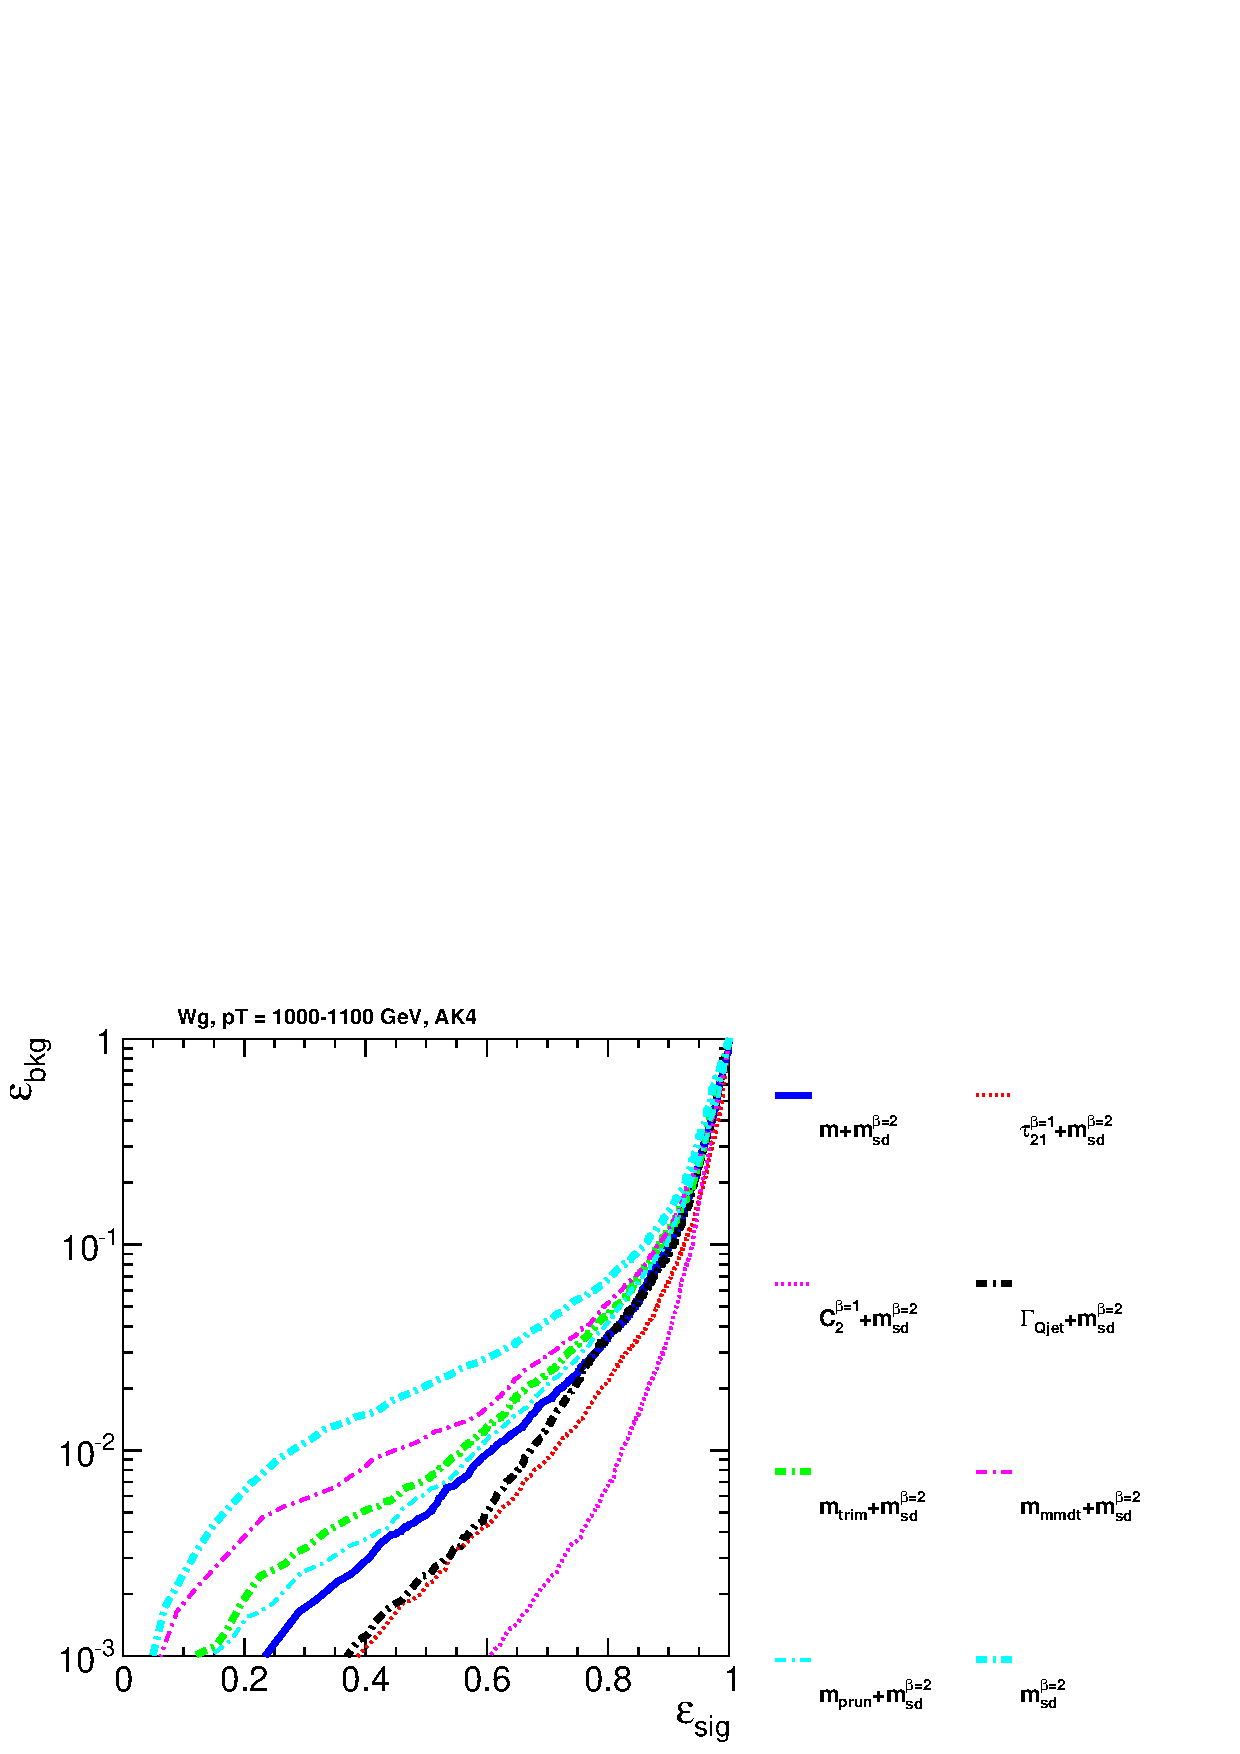
\includegraphics[width=0.48\textwidth]{./Figures/WTagging/pT500/AKtR08/Rocs_1D_j_mass_sdb2.png}}
\subfigure[mMDT mass + X]{\includegraphics[width=0.48\textwidth]{./Figures/WTagging/pT500/AKtR08/Rocs_1D_j_mass_mmdt.png}}
\caption{The BDT combinations of each mass variable with every other
variable considered in the \pt 500 GeV bin using the anti-\kT R=0.8 algorithm.}
\label{fig:pt500_masscomb_AKt_R08}
\end{center}
\end{figure*}



\subsection{Performance at High Boosts}

(this section is to cover the $W$-tagging performance for jet \pT 1-1.1 TeV and
$>$ 1.5 TeV using $\sqrt{s} = 14$ TeV samples)

{\it Maybe we don't need to divide into different medium/high boost sections.}




